%\documentclass[10pt, xcolor=x11names, compress]{beamer}
\documentclass[10pt, xcolor=x11names, compress, handout]{beamer}

\usetheme{progressbar}
%\usecolortheme[named=Purple4]{structure}
\progressbaroptions{headline=sections,titlepage=normal,frametitle=normal}

\setbeamertemplate{navigation symbols}{}

\usepackage{iwona} 

\usepackage{alltt}
\usepackage{amsmath,amsfonts, amssymb, amscd}
\usepackage{hyperref}
\usepackage{setspace}
\usepackage{wasysym}
\usepackage{ulem}

\usepackage{calc}
\usepackage[overlay,absolute]{textpos}
\TPGrid[5mm,5mm]{20}{20}



\renewcommand{\Re}{\operatorname{Re}}
\renewcommand{\Im}{\operatorname{Im}}
\newcommand{\debye}{\operatorname{debye}}

\newcommand{\chik}{$\chi(k)$}
\newcommand{\chir}{$|\tilde{\chi}(R)|$}


\newcommand{\file}[1]{{\color{Firebrick4}\texttt{`#1'}}}
\newcommand{\multiple}{{\color{Orange3}\textsl{multiple}}}


\newcommand{\atoms}  {{\color{DarkOrchid4}\textsc{atoms}}}
\newcommand{\feff}   {{\color{DarkOrchid4}\textsc{feff}}}
\newcommand{\ifeffit}{{\color{DarkOrchid4}\textsc{ifeffit}}}
\newcommand{\athena} {{\color{DarkOrchid4}\textsc{athena}}}
\newcommand{\artemis}{{\color{DarkOrchid4}\textsc{artemis}}}

\renewenvironment<>{center}
{\begin{actionenv}#1\begin{originalcenter}}
{\end{originalcenter}\end{actionenv}}

\definecolor{guessp}   {rgb}{0.64,0.00,0.64}
\newcommand{\guessp}   {{\color{guessp}guess}}
\definecolor{defp}     {rgb}{0.00,0.55,0.00}
\newcommand{\defp}     {{\color{defp}def}}
\definecolor{setp}     {rgb}{0,0,0}
\newcommand{\setp}     {{\color{setp}set}}
\definecolor{lguessp}  {rgb}{0.24,0.11,0.56}
\newcommand{\lguessp}  {{\color{lguessp}lguess}}
\definecolor{skipp}    {rgb}{0.70,0.70,0.70}
\newcommand{\skipp}    {{\color{skipp}skip}}
\definecolor{restrainp}{rgb}{0.80,0.61,0.11}
\newcommand{\restrainp}{{\color{restrainp}restrain}}
\definecolor{afterp}   {rgb}{0.29,0.44,0.55}
\newcommand{\afterp}   {{\color{afterp}after}}
\definecolor{penaltyp} {rgb}{0.55,0.35,0.17}
\newcommand{\penaltyp} {{\color{penaltyp}penalty}}
\definecolor{mergep}   {rgb}{0.93,0.00,0.00}
\newcommand{\mergep}   {{\color{mergep}merge}}


\newcommand{\fes}{FeS$_2$}
\newtheorem{conclusion}[theorem]{Conclusion}
\newtheorem{assertion}[theorem]{Assertion}
\newtheorem{exercise}[theorem]{Exercise for the reader}
\newtheorem{remember}[theorem]{Always remember}

\mode<presentation>

\title{FeS$_2$ EXAFS}%
\subtitle{The post-mortem on an Artemis demonstration}

\author{Bruce Ravel}
\institute[NIST]{Synchrotron Methods Group, Materials Measurement Science Division\\%
  Materials Measurement Laboratory\\%
  National Institute of Standards and Technology\\%
  \&\\%
  Local Contact, Beamline X23A2\\%
  National Synchrotron Light Source\\~}


\date{\today}

\begin{document}

\maketitle

\begin{frame}
  \frametitle{Copyright}
  \tiny

  This document is copyright \copyright 2007-2010 Bruce Ravel.

  \begin{center}
    
\includegraphics[width=1.0cm]{images/somerights20}
  \end{center}

  This work is licensed under the Creative Commons
  Attribution-ShareAlike License.  To view a copy of this license,
  visit \href{http://creativecommons.org/licenses/by-sa/3.0/}
  {\color{Purple4}\texttt{http://creativecommons.org/licenses/by-sa/3.0/}}
  or send a letter to Creative Commons, 559 Nathan Abbott Way,
  Stanford, California 94305, USA.

  \begin{description}
  \item[You are free:] %
    \begin{itemize}
    \item \textbf{to Share} --- to copy, distribute, and transmit the work
    \item \textbf{to Remix} --- to adapt the work
    \end{itemize}
  \item[Under the following conditions:] %
    \begin{itemize}
    \item Attribution. You must attribute the work in the manner
      specified by the author or licensor (but not in any way that
      suggests that they endorse you or your use of the work).
    \item Share Alike. If you alter, transform, or build upon this
      work, you may distribute the resulting work only under the same,
      similar or a compatible license.
    \item Any of these conditions can be waived if you get permission
      from the author.
    \end{itemize}
  \end{description}
  \begin{itemize}
  \item For any reuse or distribution, you must make clear to others
    the license terms of this work. The best way to do this is with a
    link to the URL for this document.
  \item Any of the above conditions can be waived if you get
    permission from the copyright holder.
  \item Nothing in this license impairs or restricts the author's
    moral rights.
  \end{itemize}

  Your fair dealing and other rights are in no way affected by the
  above.  This is a human-readable summary of the Legal Code (the full
  license).


\end{frame}

%%% Local Variables:
%%% mode: latex
%%% TeX-master: "pimst2"
%%% End:


\begin{frame}
  \frametitle{The amplitude parameter}
  \small%
  The amplitude parameter evaluates to something around 0.7 in the
  {\fes} fit.  This is at the low end of what is expected$^1$ for an
  $S_0^2$ parameter.  Lots of things are correlated with amplitude:
  \begin{enumerate}
  \item Coordination number, although this is a pure standard, so it
    is unlikely that coordination numbers are different from what we
    expect
  \item Sample preparation: I do not know the provenance of these
    data.  (They were taken from
    \href{http://cars9.uchicago.edu/~newville/ModelLib/search.html}
    {\color{Blue4}an on-line XAS data library}.$^2$) If the sample was
    not homogeneous, that would attenuate the amplitude$^3$ by the
    ``pinhole efffect''.
  \item Again, without knowing the provenance, I cannot comment on the
    linearity of the detectors or any other aspect of the measurement.
  \end{enumerate}

  \begin{conclusion}
    A result of $\sim0.7$ for amplitude seems acceptable.
  \end{conclusion}

  \medskip

  ~

  \begin{textblock*}{0.9\linewidth}(0pt,16.5\TPVertModule)%
    \begin{enumerate}[1.]
    \tiny%
    \item G.G.\ Li, F.\ Bridges, \& C.H.\ Booth \textit{X-ray-absorption
      fine-structure standards: A comparison of experiment and
      theory}, Phys.\ Rev.\ B \textbf{52}:9 (1995) pp\ 6332-6348.
    \href{http://dx.doi.org/10.1103/PhysRevB.52.6332}
    {\color{Blue4}\texttt{DOI:10.1103/PhysRevB.52.6332}}
  \item \href{http://cars9.uchicago.edu/~newville/ModelLib/search.html}
    {\color{Blue4}\texttt{http://cars9.uchicago.edu/~newville/ModelLib/search.html}}
  \item K.-Q.\ Lu \& E.A.\ Stern, \textit{Size effect of powdered
      sample on EXAFS amplitude}, Nuclear Instruments and Methods
    \textbf{212}:1-3 (1983) pp\ 475-478, 
    \href{http://dx.doi.org/10.1016/0167-5087(83)90730-5}
    {\color{Blue4}\texttt{DOI:10.1016/0167-5087(83)90730-5}}
  \end{enumerate}
\end{textblock*}
  
\end{frame}

\begin{frame}
  \frametitle{The $\sigma^2$ constraint on the 2$^{\mathrm{nd}}$ and
    3$^{\mathrm{rd}}$ shell S}
  \begin{columns}
    \begin{column}{0.5\linewidth}
      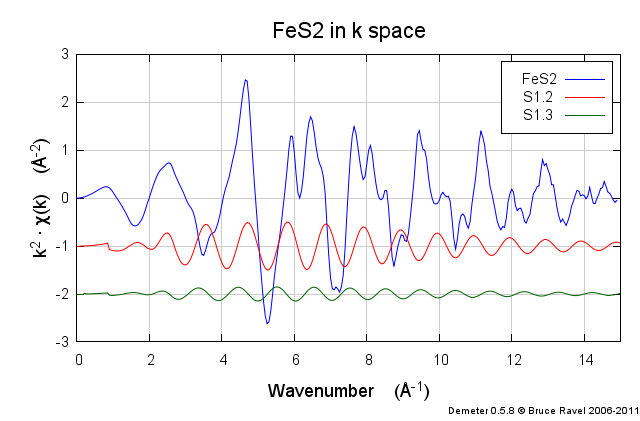
\includegraphics[width=\linewidth]{images/s2s3.png}      
    \end{column}
    \begin{column}{0.5\linewidth}
      \footnotesize%
      Here we see the contribution in $k$ of the scattering from the 6
      S atoms in the 2$^{\mathrm{nd}}$ shell and the 2 S atoms in the
      3$^{\mathrm{rd}}$ shell.

      \medskip

      These shells are separated in distance by 0.15\,\AA, which is
      just enough to have them contribute almost completely out of
      phase.

      \medskip

      This is the reason that the $\sigma^2$ parameter for the
      3$^{\mathrm{rd}}$ shell is so unreliable (indeed, negative when
      floated independently).  The fit was
      relatively insensitive to that parameter because it could reduce
      the 2$^{\mathrm{nd}}$ shell $\sigma^2$ to compensate for the
      unphysically small $\sigma^2$ from the 3$^{\mathrm{rd}}$ shell.
    \end{column}
  \end{columns}

  \begin{conclusion}
    While it is certainly unphysical to constrain these two $\sigma^2$
    parameters, the fit is more defensible with this constraint.
  \end{conclusion}
\end{frame}

\begin{frame}[fragile]
  \frametitle{That $\sigma^2$ constraint examined in detail}
  Plot the data along with a VPath (i.e.\ the sum of two or more
  regular paths) constructed from the 2$^{\mathrm{nd}}$ and
  3$^{\mathrm{rd}}$ shell S atoms.
  \begin{columns}[T]
    \begin{column}{0.5\linewidth}
      \begin{center}
        \texttt{{\color{defp}def} ss3 = ss2}
      \end{center}
      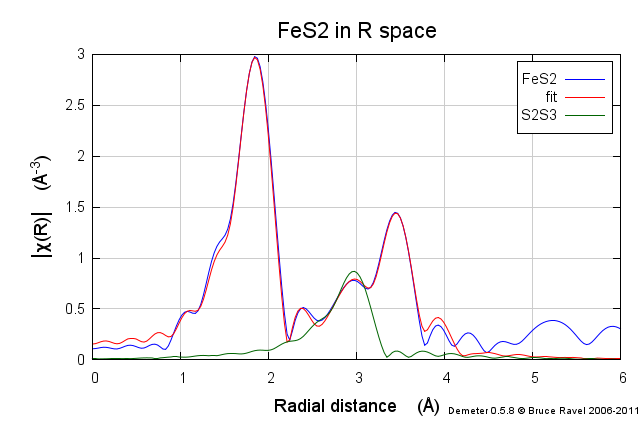
\includegraphics[width=\linewidth]{images/constrained.png}
      \tiny
\begin{verbatim}
         Number of variables         : 6
         Chi-square                  : 6104.705744295
         Reduced chi-square          : 493.543240341
         R-factor                    : 0.009268899

         ss2    =   0.00332806    # +/-   0.00130826  
         ss3   :=   0.00332806    # [ss2]
\end{verbatim}
    \end{column}
    \begin{column}{0.5\linewidth}
      \begin{center}
        {\guessp} both \texttt{ss2} and \texttt{ss3}
      \end{center}
      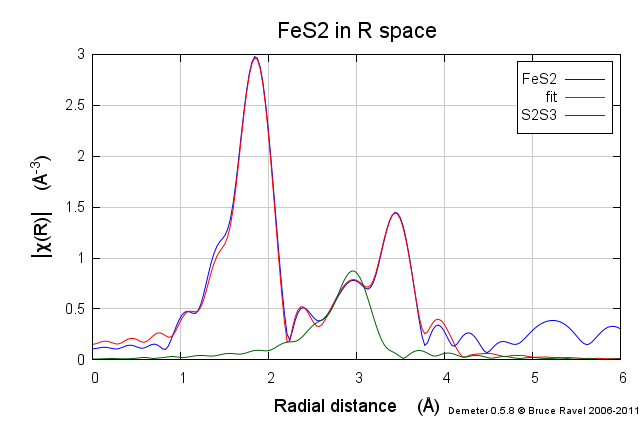
\includegraphics[width=\linewidth]{images/free.png}
      \tiny
\begin{verbatim}
         Number of variables         : 7
         Chi-square                  : 5756.383603039
         Reduced chi-square          : 506.316510008
         R-factor                    : 0.009218088  

         ss2    =   0.00270523    # +/-   0.00164548
         ss3    =   0.00014725    # +/-   0.00367061

         correlation:  ss3 & ss2  -->  0.8050  
\end{verbatim}
    \end{column}
  \end{columns}
\end{frame}

\begin{frame}
  \frametitle{The $\sigma^2$ constraints on the MS paths}
  The $\sigma^2$ parameters for the three paths involving collinear MS
  among the absorber and the 1$^{\mathrm{st}}$ shell S atoms are all
  correct.$^1$

  \bigskip

  The $\sigma^2$ parameters for the non-collinear MS paths are rather
  hokey approximations.  The problem is that we don't have a good
  model to account for the effects on $\sigma^2$ of all the legs of
  the path nor of the disorder in scattering angle.  I worry about
  introducing a new fitting parameter to account for a rather small
  effect in the data.  We need to approximate.

  \begin{assertion}
    The $\sigma^2$ constraints for the triangle MS paths are
    non-physical approximations, but are a better solution than
    floating one or more new parameters in the fit.
  \end{assertion}

  \begin{textblock*}{0.9\linewidth}(0pt,18\TPVertModule)%
    \begin{enumerate}[1.]
    \tiny
  \item E.A.\ Hudson et al., \textit{Polarized x-ray-absorption
      spectroscopy of the uranyl ion: Comparison of experiment and
      theory},\\ Phys.\ Rev.\ B \textbf{54} (1996) pp.\ 156-165
    \href{http://dx.doi.org/10.1103/PhysRevB.54.156}
    {\color{Blue4}\texttt{DOI:10.1103/PhysRevB.54.156}}
  \end{enumerate}
\end{textblock*}
\end{frame}

\begin{frame}
  \frametitle{The fourth shell S}
  Because the $\sigma^2$ for the 4$^{\mathrm{th}}$ shell S atom is so
  large, we see no improvement to the fit by introducing this
  scatterer.  

  \begin{center}
    Why is its $\sigma^2$ so large?
  \end{center}

  That's hard to say without help from theory, but clearly the
  relative positions of the absorber and this rather distant atom have
  a large thermal disorder.

  \begin{conclusion}
    It is safe to exclude this scatterer from the fit.  Indeed, the
    fit is improved by not having its frail $\sigma^2$ parameter in
    the fit.
  \end{conclusion}

  It would be interesting to measure this material at 10\,K to see if
  the signal from this distant atom could be observed.
\end{frame}

\begin{frame}
  \frametitle{The remaining MS paths}
  Nine of the first 15 paths from the {\feff} calculation were
  included in the fit.  The remaining 6 paths are MS paths with small
  amplitudes.  We got a sensible fit with a model which excluded these
  paths.  It would be a good exercise to figure out a sensible
  parameterization of their $\sigma^2$s, include them in the fit, and
  determine if the fit is improved by having them.

  \begin{conclusion}
    It was safe to exclude these paths, but this should be verified by
    examining the fits with and without those paths.
  \end{conclusion}
\end{frame}

\begin{frame}
  \frametitle{The parameterization of $\Delta R$}
  \footnotesize%
  {\fes} is a cubic crystal.  In this case, there are only two
  parameters that determine the locations of \textbf{all} the atoms in
  the cluster -- the lattice constant $a$ and the position of the S
  atom in the unit cell.  For now, we neglect the effect of  the
  position of the S atom.

  \medskip

  Why is the parameterization that sets $\Delta R=\alpha\cdot R_{eff}$
  acceptible for all paths?

  \begin{itemize}
    \footnotesize%
  \item The distance between \textit{any two atoms in a cubic crystal} is some
    geometrical factor multiplied by the lattice constant.  That
    factor depends on the positions of the atoms in the unit cell, but
    is a pure number.
  \item Thus, from the {\feff} calculation, $d_{eff}(i,j) =
    C_{ij}\cdot a_0$ for any two atoms i and j
  \item We consider an isotropic expansion (or contraction) of the
    unit, which is reasonable for a cubic lattice that does not
    undergo a phase transition.  So $a=(1+\alpha)*a_0$.
  \end{itemize}
  \begin{columns}[T]
    \begin{column}{0.15\linewidth}
      ~
    \end{column}
    \begin{column}{0.35\linewidth}
      \begin{align}
        d_{ij} =& d_{eff}(i,j) + \Delta d(i,j)\notag\\
        =& C_{ij} \cdot a \notag\\
        =& C_{ij} \cdot (1+\alpha)\cdot a_0 \notag\\
        =& C_{ij}\cdot a_0 + C_{ij}\cdot \alpha\cdot a_0\notag
      \end{align}
    \end{column}
    \begin{column}{0.35\linewidth}
      \begin{align}
        \therefore \> \Delta d(i,j) =& C_{ij}\cdot \alpha\cdot a_0\notag\\
        =& \alpha\cdot d_{eff}(i,j)\notag
      \end{align}
    \end{column}
    \begin{column}{0.15\linewidth}
      ~
    \end{column}
  \end{columns}
  \begin{conclusion}
    $\alpha\cdot d_{eff}$ works for all legs of any SS or MS path in a
    cubic crystal (if there are no internal degrees of freedom). The
    $R$ of a path is the sum of $d$ for each leg, thus $\Delta R$ for
    a path is the sum of $\Delta d$ for each leg.\\[-5.5ex]
    \begin{flushright}
      \alert{This trick is \textbf{only} valid for a cubic crystal.}
    \end{flushright}
  \end{conclusion}
\end{frame}

\begin{frame}
  \frametitle{Improving on the parameterization of $\Delta R$}
  In the crystal data for {\fes}, the S atom is at position (0.384,
  0.384, 0.384), or ($\frac{3}{8}+\delta$, $\frac{3}{8}+\delta$,
  $\frac{3}{8}+\delta$), where $\delta=0.009$.

  \medskip

  The effect of changing $\delta$ can be incorporated into the math
  expressions for $\Delta R$ for any path that includes a S atom.
  Doing so is beyond the scope of this document.

  \begin{exercise}
    Examine the \file{feff.inp} file for {\fes}.  Think about how to
    incorporate the effect of $\delta$ into a fit.
  \end{exercise}
\end{frame}

\begin{frame}
  \frametitle{Correlations}
  We have a pretty robust set of parameters in our fit.  Only two of
  the correlations are above 60\%.  

  \begin{description}[$\Delta E_0$ and $\alpha$]
  \item[$\Delta E_0$ and $\alpha$] This correlation is about 86\%.
    That is reasonable.  Those are the only two parameters effecting
    the phase of the fit.  This is a common level of correlation for
    such parameters.
  \item[1$^{\mathrm{st}}$ shell $\sigma^2$ and amplitude] This
    correlation is about 81\%.  Again, this is pretty common for two
    things that have such an effect on overall amplitude of the fit.
  \end{description}

  \begin{conclusion}
    The correlations we see are within acceptable limits.
  \end{conclusion}

\end{frame}

\begin{frame}
  \frametitle{The happiness ``parameter''}
  \small
  \begin{remember}
    Happiness is a semantic parameter and should NEVER be reported in
    a publication -- \alert{NEVER!}
  \end{remember}
  We have decades of knowledge of how the parameters of an EXAFS fit
  should behave.  ``Happiness'' attempts to encode that general
  knowledge into a single, \emph{non-statistical}, entirely semantic parameter.
  \begin{itemize}
  \item The $\mathcal{R}$-factor should be small.  An
    $\mathcal{R}$-factor below 0.02 gives no penalty. Above that, the
    penalty scales linearly to some maximum.
  \item A penalty is assessed if more than 2/3 of the number of
    independent points are used.
  \item A penalty for each Path with a negative $S_0^2$ or $\sigma^2$
    value.
  \item A penalty for each $E_0$, $\Delta R$, or $\sigma^2$ path
    parameter that is ``too big''.
  \item A penalty is assessed for each correlation above 0.95.
  \item A penalty is assessed for each non-zero restraint.
  \end{itemize}
  The evaluation of the happiness is tunable via configuration parameters.
\end{frame}

\end{document}


%%% Local Variables:
%%% TeX-parse-self: t
%%% TeX-auto-save: t
%%% TeX-auto-untabify: t
%%% TeX-PDF-mode: t
%%% End:
